\chapter{In Media We ... Trust?}

Despite the news media ecosystem's rapid evolution in the past decade, the question of fairness in reporting remains a valued one. Although counterarguments for subjective reporting exist (Glenn Greenwald, most famous for his coverage of whistleblower Edward Snowden's leaks, said that ``All journalism is a form of activism. Every journalistic choice necessarily embraces highly subjective assumptions--cultural, political or nationalistic--and serves the interests of one faction or another''), fair treatment of subjects and sources remain a central tenant to most publications \cite{Greenwald}. 
  
But an attempt at fairness on the side the reporter is not always perceived in equal effect under the eyes of the reader. Presenting contradictory facts to a reader's beliefs can even sometimes \emph{strengthen} their oppositions to it, a concept known as ``motivated skepticism'' \cite{taber2006motivated}.

In this section, we explore the theories behind three main potential sources of media distrust: In addition to the characteristics of the reader, we examine the source of the story and its use of language.


% In evolving news ecosystem, question of fairness is highly valued in the press. Most news publications have some stipulation of fairness in their handbook.
% See: Nieman Report [http://niemanreports.org/articles/fairness-in-journalism-is-rewarded/]
% Handbooks (Reuters: http://handbook.reuters.com/?title=Freedom_from_bias, NPR, etc.)

% History of press fairness: Fairness Doctrine of 1949
 
 
%Trust and fairness instead?
%Literature on Media Trust

%History of Fairness in media

%http://www.niemanlab.org/2012/06/how-do-you-tell-when-the-news-is-biased/
%the cool experiment
 
 
 
 

\section{What You Read is Who You Are}

It comes as no surprise that our own political stances have a significant effect in our perceptions of bias in the media. 

In even seemingly neutral stories, partisans tend to view reporting as biased against their own views. This phenomenon---deemed the ``hostile media effect''---was first studied at Stanford University by Robert P. Vallone, Lee Ross, and Mark R. Lepper in 1985 \cite{vallone1985hostile}. Although ``true'' neutrality of a story is nearly impossible to quantify due to the subjective nature of the concept, Vallone et. al were able to successfully demonstrate that partisans of \emph{both} sides (pro-Israeli and pro-Arab) viewed the same news segments as hostile towards their beliefs and favorable to the other side.

%? Perceptions of media bias, then, have as much to do as self-serving motivations to secure preferential treatment as they do with the media itself.
  
%? The political leanings of the reader are essential considerations when attempting to measure other factors that contribute to bias. In 

\section{Who You Read is What You Are}




%The media, of course, is not just one unified mass, and in an increasingly fragmented ecosystem, the role of media brands is a crucial factor in the perception of bias. Although most research
%\cite{baum2008eye}


 
%For instance, most research on the hostile media phenomenon conceptualizes the news media as an undifferentiated mass of information sources that individuals can (and do) reasonably characterize as having a uniform political orientation (Giner-Sorolla and Chaiken 1994, Peffley et al. 2001, Eveland and Shah 2003). Yet, the past two decades have seen a dramatic increase in the number and variety of news sources. One consequence is that Democrats and Republicans are increasingly likely to differ systematically in their assessments of specific media outlets.






%With the decline of print newspapers, a diverse number of new platforms and web-centric publications have risen.


%How do you control for the above things in your study?

\section{The Role of Language [Policial Persuasion]}




\subsection{Language and Politics}
%Presidential speeches degrading over time-- ie simple language appeals to the masses in politics
\subsection{The Seductive Allure [... of Simple] Language}
%But we trust complex language for explaining technical facts

%Test image

%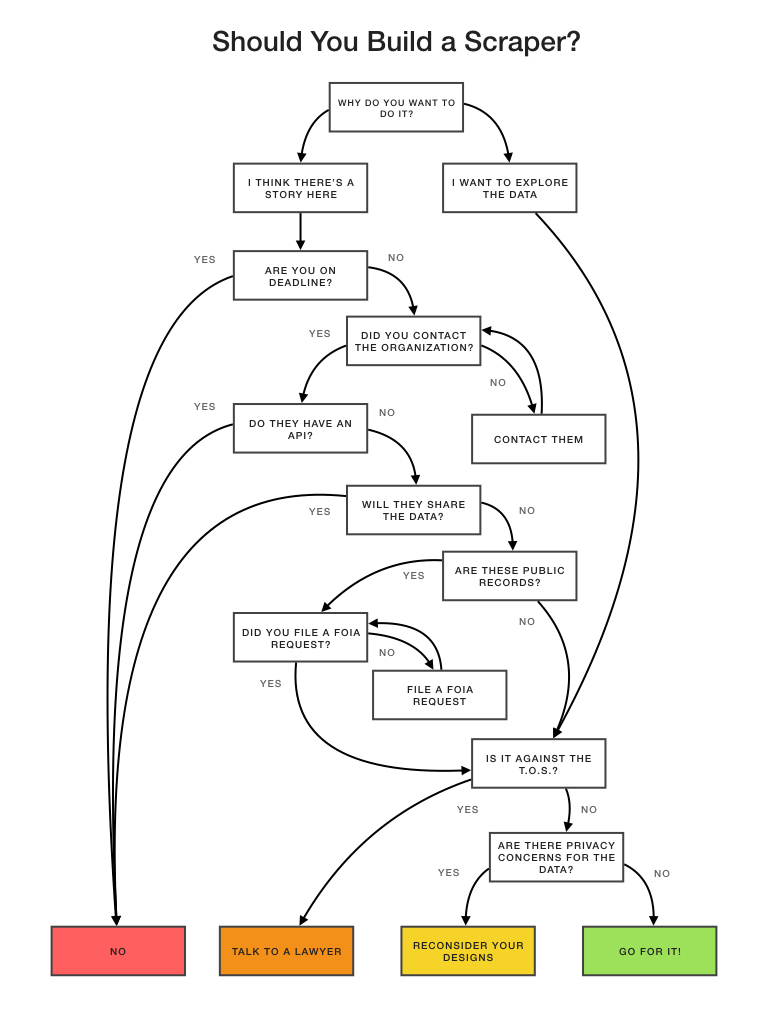
\includegraphics[width=\textwidth]{flowchart_final}

  







